% Upload the two PDFs to the figures/ folder in your EXISTING Overleaf project.
% Paste these figure environments where the new experiments are discussed.
% These captions do not change the definitions or results of the original tasks.

\begin{figure}[tbp]
  \centering
  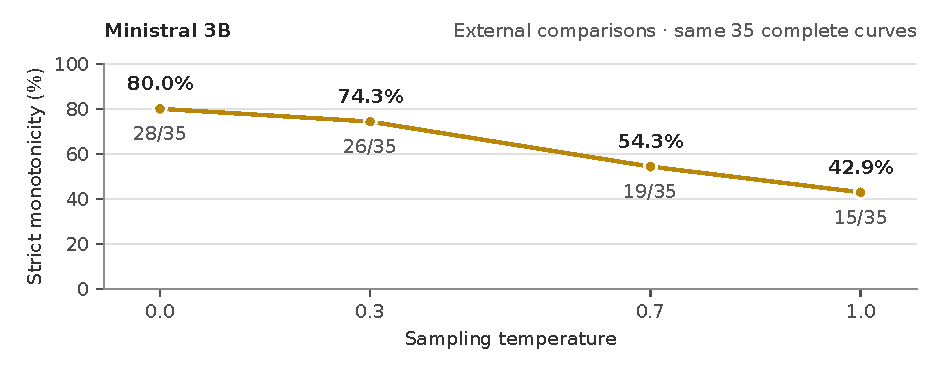
\includegraphics[width=\linewidth]{figures/ministral_temperature_monotonicity.pdf}
  \caption{Temperature sensitivity in a Ministral 3B pilot. We compared
  the seven tiers of 12 ladders against three shared comparison statements,
  using 20 choices per tier--statement pair (10 in each presentation order).
  The plot uses the same 35 complete curves at all four temperatures.
  One failed request at temperature 0.7 left one of the 36 planned curves
  incomplete; that curve is excluded at every temperature.
  Labels give the percentage and number of curves with no downward step.
  Higher temperature did not improve observed strict monotonicity in this pilot.
  These are descriptive results: curves share ladders and comparison statements,
  and the scores do not determine whether underlying preferences are coherent.}
  \label{fig:ministral_temperature}
\end{figure}

\begin{figure}[tbp]
  \centering
  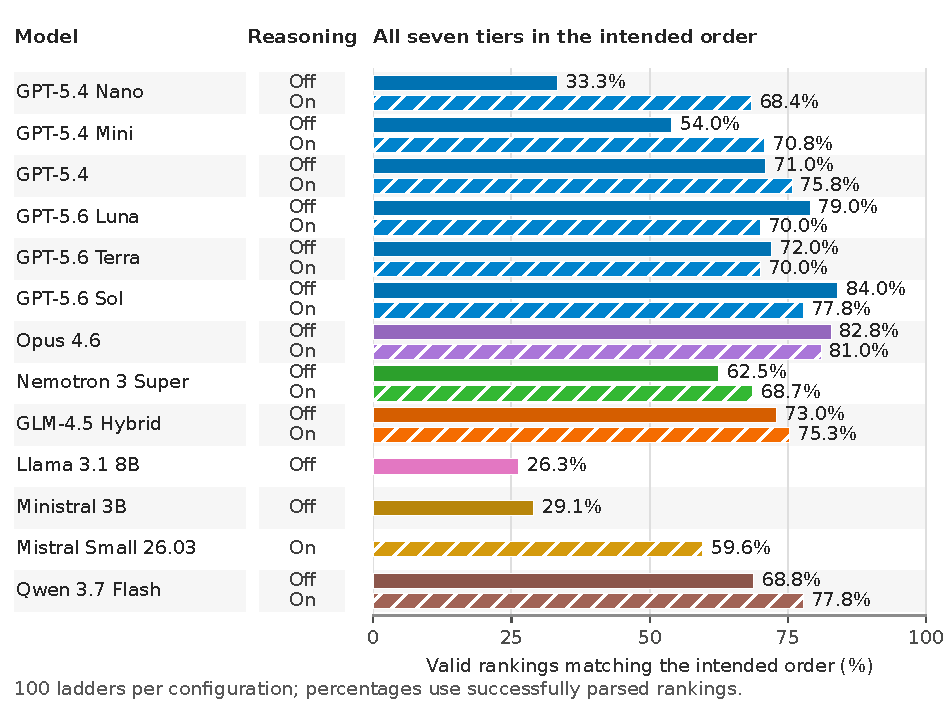
\includegraphics[width=\linewidth]{figures/full_ladder_ranking.pdf}
  \caption{Direct ranking of all seven statements in each of the 100 canonical
  ladders, evaluated separately from the pairwise and external-comparison tasks.
  Each configuration received one request per ladder, with the same seeded
  shuffle of the statements across configurations. Exact order match is the
  percentage of valid rankings that reproduce the full intended tier ordering.
  Each bar shows this percentage, with the reasoning setting labeled beside it.
  A ranking counts as an exact match only if all seven tiers appear in the
  intended order. Scores use the original parser and the number of valid
  rankings for each configuration, ranging from 86 to 100.
  Of 2,300 requested rankings, 2,241 were
  valid under this parser. An additional 33 were recoverable by a separate
  formatting check and are not included here. On/off denotes the reasoning
  setting. This task measures agreement with the intended ordering; requesting
  a single complete ranking does not independently test transitivity.}
  \label{fig:direct_ladder_ranking}
\end{figure}
